\documentclass[../main.tex]{subfiles}

\begin{document}

\chapter{Evaluation}

This chapter evaluates the protocol proposed in chapter~\ref{chap:design}.
Besides the verification of the intended functionality in section~\ref{sec:evaluation-func}, the security and performance of the protocol are investigated in sections \ref{sec:evaluation-sec} and \ref{sec:evaluation-perf}.
This evaluation verifies that the system requirements given in section~\ref{chap:requirements} can be fulfilled.

\section{Functionality}
\label{sec:evaluation-func}

This section evaluates the functionality of the designed protocol.
Specifically, the protocol must ensure that the data owner can always access its logs.
The data owner must also be able to share and revoke access to logs.
Please see section~\ref{functional-requriements} for details about those functional requirements.

To ensure that data owner can always access logs the protocol relies on three mechanisms:
First, the monitor must encrypt a new log only for the data owner.
A log is therefore accessible for the data owner upon creation.
Second, whenever the data owner shares or revokes access to a log it must include its own identity in the set of authorized users.
Finally, the server must ensure that no other user besides the data owner can modify logs.
Since no unauthorized users can tamper a log this guarantees that that the data owner is always able to download and decrypt its logs.

The protocol is based on hybrid encryption.
This means that the log is first encrypted with a symmetric encryption scheme.
The used symmetric key is then encrypted for each intended recipient.
Those encrypted keys are attached to the encrypted log.
This allows the construction of logs that can be decrypted by multiple users.
Hence, a data owner can re-encrypt the log for a specific set of users by applying the encryption algorithm.
The specified metadata allows the server to distribute logs to requesting users because it contains the set of intended receivers.
Moreover, the server can ensure that only the specified data owner can update a log.
This effectively enables the functionality to share and revoke access to the log.
Sharing a log is realized by adding additional users to the set of authorized users.
Revoking the access to logs requires to remove a user from this set.
Since new key material is generated during encryption, revoked users can not re-use older decryption keys to access the log.

This analysis shows that the designed protocol fulfills all identified functional requirements.
A data owner can always access its logs and it can share and revoke access to them.
The protocol was included in the existing toolchain within the scope of the master thesis.
Section \ref{sec:toolchain-modifications} investigates the implemented changes.
This integration verifies that the protocol has the intended functionality and can be used in practice.
Moreover, the implemented libraries are heavily tested.
This creates further confidence in their functionality.

\section{Security}
\label{sec:evaluation-sec}

This section investigates the security of the designed protocol.
Three security requirements were identified during requirements engineering (details in section ~\ref{security-requriements}).
Each requirement was motivated by an exemplary attack scenario.
The following sections face the proposed protocol with those attacks.
They argue why the established security mechanisms resist them.

\subsection{Assumptions}

The security of the protocol relies on three fundamental assumptions.
If any of those assumptions is broken the protocol must be considered to be insecure.

\begin{enumerate}
    \item 
    The protocol has access to a secure PKI.
    The PKI assigns the identities of users to their public keys via certificates.
    Each user requires two key pairs (one for encrypting data and one for signing data).
    Each user must has exclusive access to his private keys.
    The public keys are distributed via certificates which are signed by a trusted certificate authority.
    If any private key (either of a user or of the certificate authority) is compromised the intended E2EE is broken.
    A private key is assumed to be compromised if any entity besides the owner of the private key has access to it.
    
    \item 
    The JOSE standard provides secure encryption and signing algorithms.
    Specifically, \verb|A256GCM| and \verb|ECDH-ES+A256KW| must be secure encryption algorithms and \verb|ES256| must be a secure signing algorithm.
    This implies that it is computationally infeasible to break those algorithms without knowing the respective keys~\cite{Katz2020}.
    \item 
    The libraries implemented in this thesis rely on language-specific JOSE implementations (details in~\ref{sec:implemented-libraries}).
    It is crucial for the security of the protocol that those libraries follow the specifications and definitions of the JOSE protocol.
\end{enumerate}

\subsection{Curious server}
A curious server is a passive attacker which tries to access the logs within the toolchain.
It motivated security requirement S1 which states that only the data owner and explicitly authorized users can access logs.
Recall the attacker Eve who is the database admin of the Overseer server.\todo{cite section}
This section argues why Eve can not access logs if he was not explicitly authorized.

The protocol enforces that only encrypted data is stored in the database.
Both, the monitor creating a log and the data owner sharing a log must encrypt the data before sending it to the server.
The server only has access to the \emph{JWE} token created by the encryption algorithm.
This \emph{JWE} token relies on hybrid encryption:
First, a symmetric key $k$ is randomly generated and the data is encrypted via \verb|A256GCM|.
This is an authenticated symmetric encryption algorithm based on \emph{AES}~\cite{Jones2015}.
Secondly, this symmetric key $k$ is encrypted for each receiver using \verb|ECDH-ES+A256KW|~\cite{Jones2015}.
This key wrapping algorithm establishes an ephemeral key between two users.
This ephemeral key is finally used to encrypt the symmetric key $k$.
The specification of \verb|ECDH-ES+A256KW| requires the following steps to establish this ephemeral key between a sender and receiver~\cite[100]{Barker2017}.
This is also illustrated in figure~\ref{fig:key_wrapping}.

\begin{figure}[ht]
    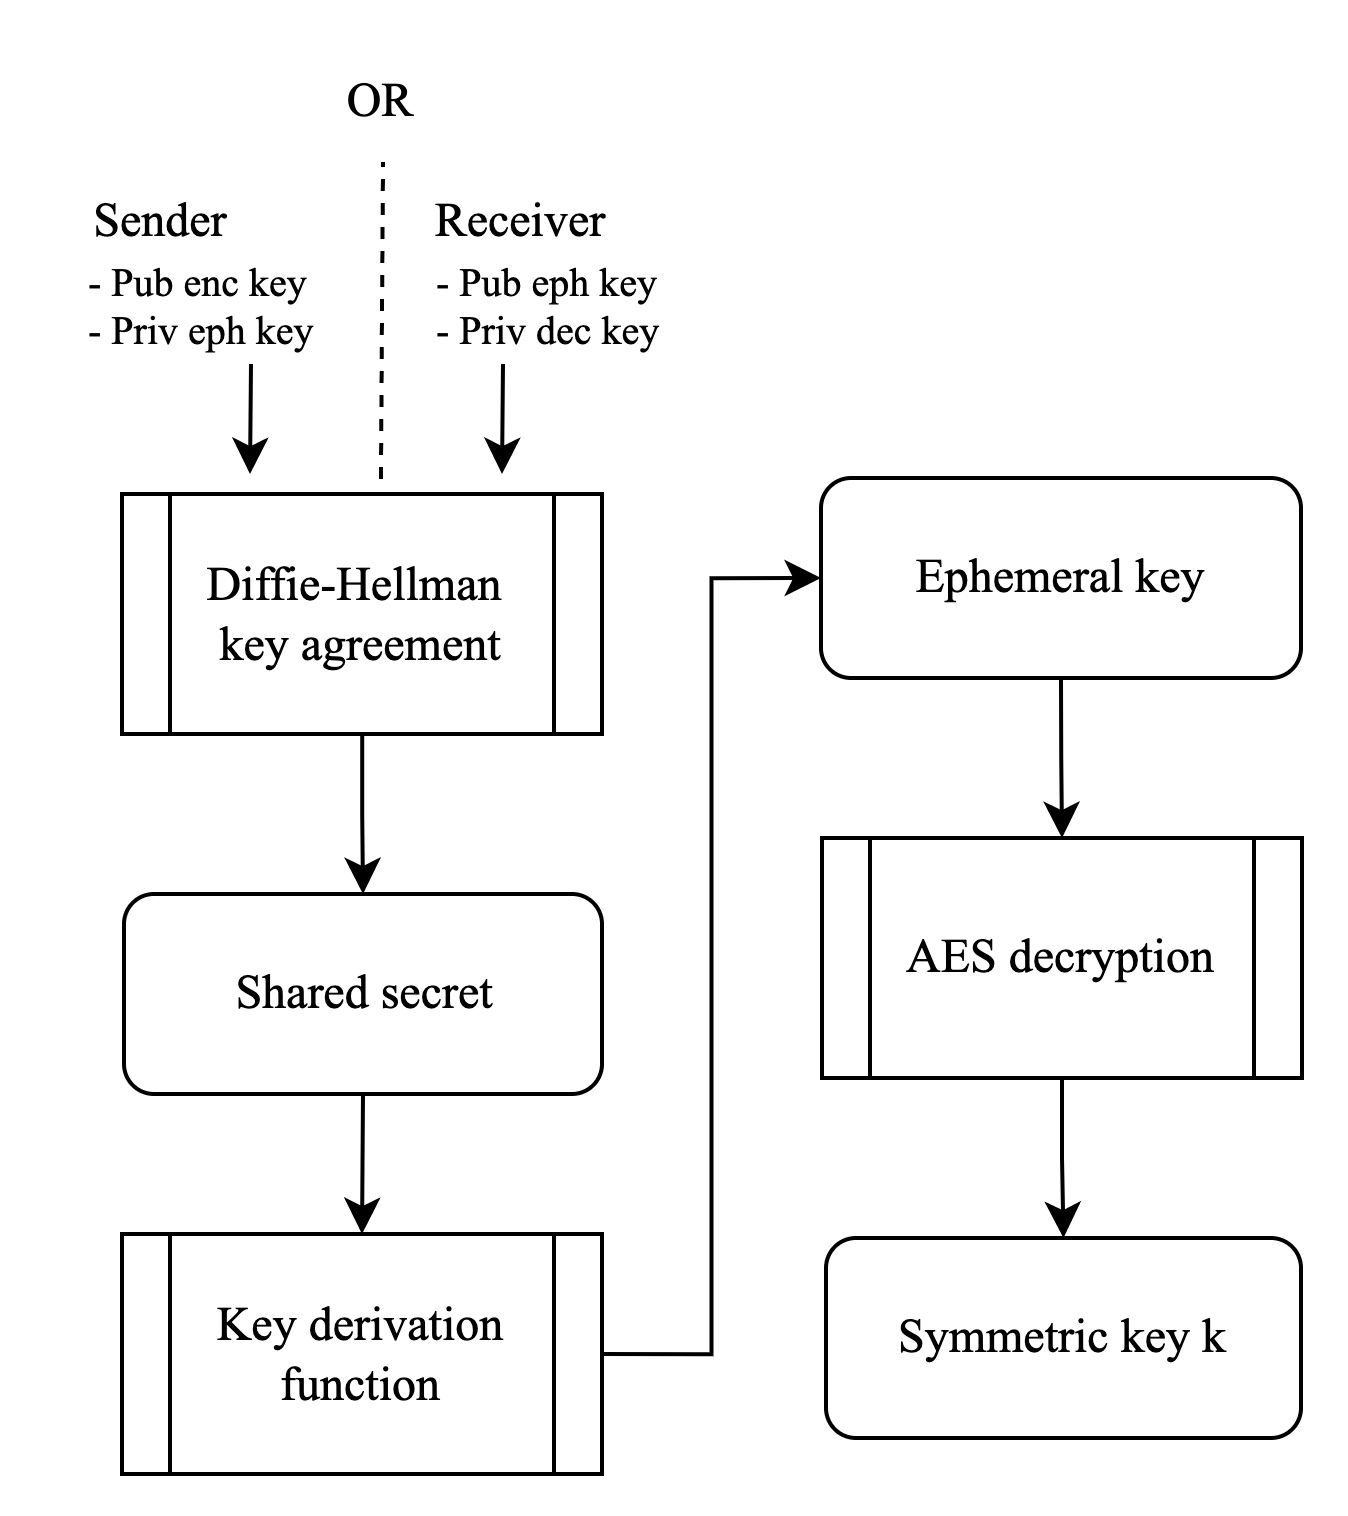
\includegraphics[scale=0.2]{../img/07/key_wrapping.jpg}
    \centering
    \caption[Key wrapping]{
        Key wrapping of the symmetric key k using ECDH-ES+A256KW. 
        Based on the exchanged public keys the sender and receiver can both compute the same shared secret.
        The derived ephemeral key is finally used to decrypt the symmetric encryption key k.}
    \label{fig:key_wrapping}
\end{figure}

\begin{enumerate}
    \item 
    The sender must know the static public key of the receiver. 
    In our case, this is the public encryption key.
    The receiver must have exclusive access to its static private key.
    In our case, this it the private decryption key.
    \item 
    The sender creates a new ephemeral key pair. 
    This key pair must be used only once.
    \item 
    The sender sends the ephemeral public key of to the receiver.
    In our case, the key is encoded into the \emph{JWE} token.
    The ephemeral private key must be kept secret.
    \item 
    The sender knows the static public key of the receiver and the ephemeral private key of the sender.
    The receiver knows the ephemeral public key of the sender and the static private key of the receiver.
    Thus, the Diffie-Hellman key agreement protocol can be used to compute a shared secret between the sender and the receiver~\cite[section 9.3.6]{Eckert2018}.
    The computation of the shared secret requires either the ephemeral private key or the static private key.
    If both are kept secret it is assumed to be computationally infeasible to compute the shared secret~\cite[section 9.3.6]{Eckert2018}.
    \item 
    The shared secret (which is the result of the Diffie-Hellman key agreement protocol) is finally used as input for a key derivation function.
    This function finally computes the ephemeral key between the sender and the receiver.
\end{enumerate}

To access a decrypted log the attacker Eve needs to have access to the symmetric key $k$.
This requires him to decrypt any of the encrypted keys attached to the \emph{JWE} token.
To succeed, Eve must have access to any of the ephemeral keys which were used to encrypt $k$.
Eve can compute an ephemeral key only if he has access to either the ephemeral private key of the sender or the static private key of the receiver.
However, those private keys must be kept secret.
If Eve wants to decrypt the log he must either break the encryption algorithms or access a private key.
This, however, contradicts the assumptions.
If Eve can break the encryption the used encryption algorithm it is not secure.
If Eve can access a private key of a user the PKI is not secure.
This leads to the conclusion that the malicious database admin Eve can not access decrypted logs.
Only if he was explicitly authorized he can restore the symmetric key $k$ which allows the decryption of a log.


\subsection{Surreptitious forwarding}
Surreptitious forwarding refers to an attack where a malicious user re-encrypts a received log for unintended users (details in section~\ref{sec:surreptitious-forwarding}).
Since such attacks must be detected the security requirement S2 was introduced.
Receivers of encrypted logs must be able to verify that the log was intentionally shared with them.
Recall the attacker described in \todo{cite section}.
Alice shares a log with Eve.
This implies that Eve has access to the decrypted data.
Eve, however, does not stick to the protocol and encrypts the received log for Bob.
Bob must be able to detect this fraud because the log he received was not encrypted by the data owner (Alice).
This section argues why the designed protocol can detect this attack.

The construction introduced to defend against this attack is the shared log.
It is a \emph{JWS} token that is signed by the creator of the log.
For details see the visualization in figure~\ref{fig:nested-jws}.
A shared log contains the log as a nested \emph{JWS} token.
Moreover, it contains the identity of the creator and the identities of the intended receivers.
Whenever a user successfully decrypted a log, it must verify that the shared log is a valid data structure.
This requires the following checks:
\begin{enumerate}
\item 
First of all, the receiver needs to verify if the shared log was signed by the claimed creator.
It fetches the public key of the claimed creator and verifies the cryptographic signature.
If the signature is valid the receiver can be sure that the log was signed by the private signing key of the creator.
\item 
The receiver then needs to check if the creator is the data owner. 
This is achieved by checking if the identity of the creator (shared log) is equal to the identity of the data owner in the nested log.
If this holds and if the log was indeed signed by a valid monitor the receiver can be sure that the data owner created and signed the shared log.
This, however, does not prevent surreptitious forwarding.
\item 
In a third step, the receiver must verify if his identity is specified in the list of intended receivers (shared log).
If this is true the receiver knows that the data owner intentionally shared the log with him or her.
This follows from two observations:
First, the receiver can be sure that the shared log was indeed created by the data owner.
Second, the receiver knows that the data owner included his identity in the set of intended receivers.
This gives the receiver confidentiality that no malicious entity re-encrypted the log for him or her.
\end{enumerate}

The following consequence can be observed from this validation:
The creator specified in the shared log must have signed the shared log.
The creator specified in the shared log must be equal to the data owner.
Thus, the shared log is only valid if the data owner has shared the signed log.
Eve has two options to forward an encrypted log to the unintended receiver Bob. 
\begin{itemize}
    \item 
    He could manipulate the identity of the data owner.
    If he manages to change the identity of the data owner to its own identity he could correctly sign the shared log.
    This modification, however, makes his attack pointless.
    Eve does not want to introduce faked logs.
    He wants to forward existing logs to unintended receivers.
    Please also note that this requires Eve to be a valid monitor because only they are allowed to sign logs.
    \item 
    He could try to forge a signature of the data owner Alice.
    This does not require him to modify the log.
    Rather, Eve keeps the existing log and creates a shared log that includes Bob as a valid receiver.
    He also specifies Alice as the creator of the shared log.
    This approach requires Eve to create a signature in the name of Alice because Bob will check if the claimed creator signed the shared log.
    However, this contradicts the assumptions:
    To successfully forge a signature Bob either has access to the private signing key of the data owner or he breaks the signing algorithm.
    The former breaks the security of the assumed PKI.
    The latter breaks the security of the chosen signing algorithm.
\end{itemize}

This analysis shows that there is no way for Eve to forward a received log to unintended recipients if those recipients validate the shared log correctly.


\subsection{Malicious data owner}
A malicious data owner is a user trying to modify existing logs or create arbitrary new logs.
It then tries to share the forged log with other users in the system.
Security requirement S3 was introduced to defend against this attack.
This section elaborates on how recipients of shared logs can detect this fraud.

The designed protocol defines a log as a cryptographically signed data structure.
Each log must be signed by a valid monitor.
The protocol also requires the validation of this signature during decryption.
In particular, a receiving user must perform the following tasks to ensure the validity of the log:
\begin{enumerate}
    \item 
    The monitor specified within the log must have signed the log.
    This requires the receiver to download the public verification key of the claimed monitor.
    The receiver can be sure that the log was signed by the private key of the monitor if the verification succeeds.
    \item 
    The receiving user must also validate that the claimed monitor is allowed to create logs.
    Otherwise, arbitrary users could sign logs.
    This requires the installed PKI to deliver this information, e.g. by encoding it into the certificates of the monitor components.
\end{enumerate}

Consider Eve to be a malicious data owner trying to share a forged log.
First of all, Eve creates his malicious log data.
He then needs to sign this data using the private signing key of the monitor specified in the log.
Otherwise, the recipient would notice that the claimed monitor did not sign the log.
Eve has two options.
First, he could specify his identity and sign the log with his private signing key.
Eve must be a valid monitor because otherwise, the recipient would detect the fraud.
Second, Eve could specify an existing monitor in the log.
This passes the check if the claimed monitor is allowed to create logs.
However, it requires Eve to create a signature in the name of the monitor which contradicts the assumptions.
Either he needs access to the private signing key of the claimed monitor (insecure PKI) or he needs to break the signing algorithm (insecure algorithm).
Both options are not feasible under the given assumptions.
Thus, a malicious data owner Eve can not introduce forged logs into the system.

\section{Performance}
\label{sec:evaluation-perf}
As elaborated in the previous chapters, the designed and implemented protocol is based on hybrid encryption.
Logs can therefore  be encrypted for multiple recipients.
The symmetric key $k$ (which encrypts the log) must be encrypted for each receiver.
This implies that if a log is shared with $n$ users the key $k$ must be encrypted $n$ times.
The encryption duration increases linearly with the number of recipients.
This section aims to provide resilient measurements of those costs.


\subsection{Methodology}
The encryption times are measured for each library separately (ts-it-crypto, py-it-crypto and go-it-crypto).
The measurements are implemented as performance tests in each library.
All of them follow the same principles.
The encryption duration is quantified by measuring the passed milliseconds during encryption.
Always the same log data is encrypted.
However, the number of recipients changes during different tests.
For a fixed number of recipients a tests is repeated $100$ times.
The average of those runs is said to be the encryption duration for the number of recipients in the library under test.

The performance tests were executed on a machine running \emph{macOS Monterey} with an \emph{Apple M1} CPU (ARM64).
The Go library was compiled with Go 1.18.3\footnote{\url{https://go.dev/doc/devel/release}}.
The Typescript package was compiled to Javascript using TSC 4.8.3\footnote{\url{https://www.typescriptlang.org/docs/handbook/compiler-options.html}}. 
It was then executed by the Node.js version 18.12.1\footnote{\url{https://nodejs.org/ca/blog/release/v18.12.1/}} which is built upon the V8 engine 10.2.154.15\footnote{\url{https://v8.dev/}}.
The Python tests were run under Python 3.9.6\footnote{\url{https://www.python.org/downloads/release/python-396/}} using the CPython\footnote{\url{https://github.com/python/cpython}} interpreter.

\subsection{Results}
The results of all three libraries are illustrated in figure~\ref{fig:performance}.
It shows the encryption duration in milliseconds for a different number of recipients.
In general, one can observe that the Go implementation is the fastest library.
This meets the expectations because Go is a compiled language while Python and Typescript are interpreted.
Please note that Typescript is compiled into Javascript.
The resulting Javascript code, however, is also interpreted by the V8 engine included in Node.js.
The performance difference between the Python and Typescript implementations is remarkable.
Both rely on the native OpenSSL module installed on the operating system.
Hence all complex cryptographic tasks are computed by pre-compiled libraries.
This improves the performance of both libraries.
The observed speed difference can be explained best when considering the performance differences between the Javascript engine V8 and the CPython interpreter:
The experiments performed by~\cite{Lion2022} indicate that execution times under V8 are on average almost four times faster than under CPython.

For all languages one can observe a linear growth of encryption times when adding additional recipients.
This meets the expectations because all libraries rely on hybrid encryption.
When adding a new user the encrypting party must additionally encrypt the secret key for this user.
The encryption for a single receiver in Go takes $0.12ms$.
The encryption for two receivers takes $0.17ms$.
The additional receiver increases the costs by a about $0.05ms$ because both runs encrypted the same log.
The same analysis can be done for the Python and Typescript measurements.
While an additional recipient in Python increases the encryption costs by approximately $0.50ms$, the Typescript implementation requires about $0.30ms$ for an additional user.

From the perspective of a user, a system reacts instantaneously if a computation takes less than $100ms$~\cite{Nielson1993}.
In those cases no visual feedback is necessary.
Experiments with the packages show that this treshold is reached in Typescript if encrypting the log for about $330$ users.
The Python implementation reaches the boundary if data is encrypted for $170$ users.
In Go the encryption for $1500$ recipients takes on average slightly more than $100ms$.
This proofs that a data owner can share his logs with up to 170 users without noticing a computation delay.
Hence, the designed protocol can be used in practice.




\begin{figure}[ht]
    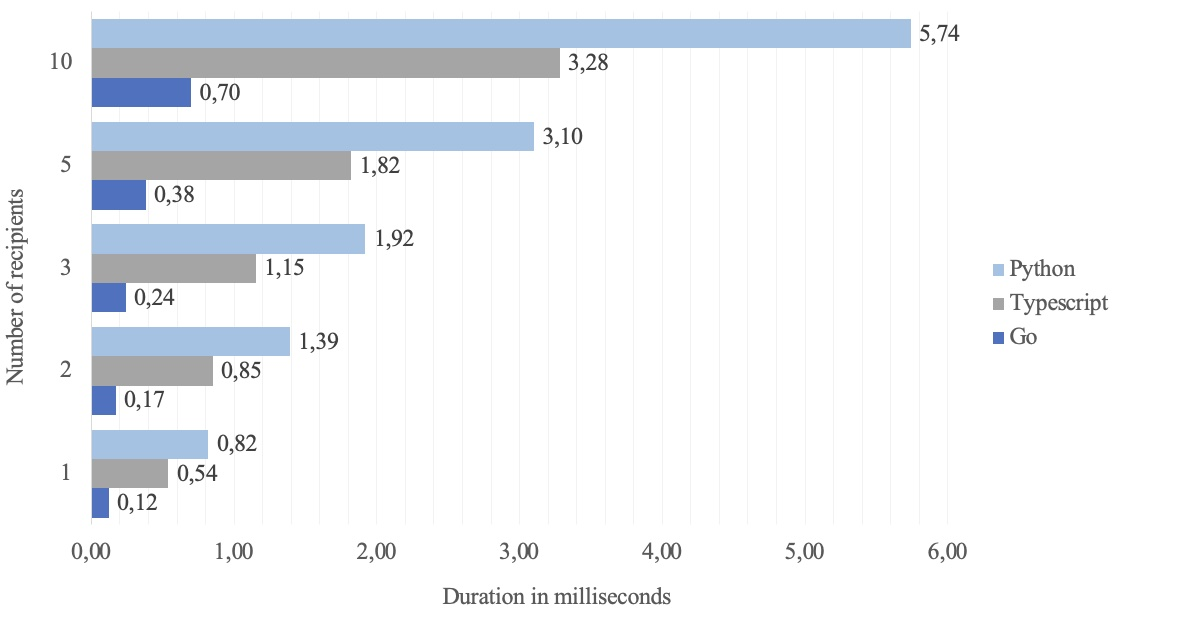
\includegraphics[scale=0.3]{../img/07/performance_tests.jpg}
    \centering
    \caption[Encryption duration]{This figure visualizes the encryption duration of the different libraries in milliseconds. The same log data was encrypted for a different number of recipients.}
    \label{fig:performance}
\end{figure}

\end{document}